\documentclass[11pt]{article}
% Reproducible PDF: no creation or modification date and a fixed trailer ID.
\ifdefined\pdftrailerid
  \pdfinfoomitdate=1
  \pdftrailerid{}
\fi
\usepackage[T1]{fontenc}
\usepackage{lmodern}
\usepackage[margin=1in]{geometry}
\usepackage{amsmath,amssymb}
\usepackage{booktabs}
\usepackage{graphicx}
\usepackage{enumitem}
\usepackage{microtype}
\usepackage{xcolor}
\usepackage{caption}
\usepackage[numbers,sort&compress]{natbib}
\usepackage[hidelinks]{hyperref}

\captionsetup{font=small,labelfont=bf,skip=6pt}
\setlist{itemsep=2pt,topsep=4pt}
\newcommand{\todo}[1]{\textcolor{red!70!black}{[TODO: #1]}}
% generated by make_tables.py from committed results; do not edit
\newcommand{\EegFCeight}{81--86}
\newcommand{\EegLeight}{64}
\newcommand{\EegFCsixteen}{65--75}
\newcommand{\EegLsixteen}{46}
\newcommand{\EegFCthirtytwo}{48--64}
\newcommand{\EegLthirtytwo}{23}
\newcommand{\EegNFeight}{19}
\newcommand{\EegTFeight}{5--7}
\newcommand{\EegQeight}{17}
\newcommand{\EegQL}{16\%, 18\% and 16\%}
\newcommand{\EegRsaFCeight}{62--72}
\newcommand{\EegRsaLeight}{55}
\newcommand{\EegRsaNFeight}{2.0}
\newcommand{\EegCells}{10}
\newcommand{\EegBias}{$-0.008$}
\newcommand{\EegKtwentyFC}{49--63}
\newcommand{\EegKtwentyL}{31}
\newcommand{\EegPcaFC}{51--64}
\newcommand{\EegPcaL}{44}
\newcommand{\MouseFCeight}{100}
\newcommand{\MouseLeight}{99.7}
\newcommand{\MouseLsixteen}{97.7}
\newcommand{\MouseNFeight}{16}
\newcommand{\MouseQeight}{16}
\newcommand{\MouseQL}{15\% and 16\%}
\newcommand{\MouseRsaFCeight}{100}
\newcommand{\MouseRsaLeight}{100.0}
\newcommand{\MouseRsaNFeight}{0.9}
\newcommand{\MouseCells}{12}
\newcommand{\MouseBias}{$+0.003$}
\newcommand{\MouseTFmax}{1.4}
\newcommand{\MouseUnwhitenedNF}{46}
\newcommand{\EegUnwhitenedFC}{100}
\newcommand{\RatioEeg}{0.92}
\newcommand{\RatioMouse}{0.24}
\newcommand{\RelEeg}{0.88}
\newcommand{\RelMouse}{0.73}
\newcommand{\PosMouse}{94}


\title{Most faithful-looking neighborhoods in 2-D maps\\ of trial-averaged neural responses are spurious}
\author{Sooyoung Jang\\[2pt] \small Hanbat National University\\ \small\texttt{syjang@hanbat.ac.kr}}
\date{Draft, October 2026}

\begin{document}
\maketitle

\begin{abstract}
Two-dimensional maps of trial-averaged responses, made with t-SNE or multidimensional scaling
(MDS), are often read neighbor by neighbor. A natural safeguard is to check whether a point's
displayed neighbors are also its neighbors in the full-dimensional averaged data. We ask how
often a neighborhood that passes this check is faithful to the noise-free responses that the
averages estimate. The share of passing neighborhoods that are not faithful we call
\emph{false comfort}. We estimate it from held-out repetitions, with a
simulation--extrapolation-type correction for the reference's own noise. The analyses were
fixed in advance and run on two independent datasets: human EEG (THINGS-EEG2; 10 subjects,
200 images, 80 repetitions) and two-photon imaging of mouse primary visual cortex (Allen Brain
Observatory; 10 mice, 118 images, 50 repetitions). With 8 trials averaged, \EegFCeight\% of
the neighborhoods that passed the check were not faithful in EEG (conservative bound
\EegLeight\%). In mouse V1 essentially all were (bound \MouseLeight\%). Maps of
cross-validated distances passed far fewer neighborhoods, but those were mostly unfaithful
too. The result held in \EegCells{} of 12 pre-specified variations in EEG and in all 12 in
mouse V1. In
exploratory analyses, the severity tracked the ratio of neighbor distances to the noise of the
trial averages: \RatioEeg{} in EEG and \RatioMouse{} in mouse V1. Local neighborhoods in such
maps should not be read without a reference built from held-out repetitions.
\end{abstract}

\section{Introduction}

Two-dimensional maps of condition-averaged responses are a staple of systems neuroscience.
Representational similarity analysis displays condition means with MDS
\citep{kriegeskorte2008,nili2014}, object spaces are shown the same way \citep{hebart2023}, and
t-SNE \citep{vandermaaten2008} maps of population responses are common. Such maps are read
locally: two images that sit together are taken to evoke similar responses.

It is well documented that 2-D maps distort the neighborhoods of the data they are fitted to
\citep{chari2023,cooley2019,lause2024}. Quality criteria measure how well a map preserves those
neighborhoods \citep{lee2009,venna2010}. It is also known that judging a map against noisy data
can mislead: hyperparameters chosen for fidelity to the data overfit its noise, and maps are
better judged against a denoised signal \citep{lin2024}.

This note asks a narrower, practical question. After averaging trials, an analyst can check
each displayed neighborhood against the averaged data, and a neighborhood that passes looks
trustworthy. But the averages carry noise, and the map was fitted to the same noisy averages.
The check therefore shares its errors with what it checks. This is the conditional dependence
that makes a diagnostic test look accurate against a reference with correlated errors
\citep{vacek1985}. How often, then, is a neighborhood that passes the check not faithful to the
noise-free responses?

We define this rate of \emph{false comfort} and estimate it from held-out repetitions. The
estimator is not new in kind. It is the classification accuracy of a decision made from noisy
scores, judged against true scores \citep{livingston1995}. The reference's own noise is removed
by a simulation--extrapolation-type step \citep{cook1994,devanarayan2002}. What is new is its
application to the neighborhoods of 2-D maps. The claims, thresholds and variations were fixed
before the analyses were run.

\section{Neighborhood labels and false comfort}\label{sec:def}

Objects $i=1,\dots,n$ (stimuli) have noise-free mean responses $\mu_i\in\mathbb{R}^D$ in a fixed
representation. An analyst averages $R$ repetitions into $c_i$, fits a 2-D map to the $c_i$, and
reads the set $E_i$ of the $k$ points nearest to $i$ in the map. For $j\in E_i$, let
$\mathrm{rank}_i(j)$ be the position of $j$ among all objects ordered by their distance
$\|\mu_i-\mu_\ell\|$ from $i$. The \emph{reach} of $i$ is the $\lceil(1-\varepsilon)k\rceil$-th
smallest of these ranks, and the displayed neighborhood is \emph{faithful at tolerance $k'$} if
its reach is at most $k'$: at least $\lceil(1-\varepsilon)k\rceil$ of the $k$ displayed neighbors
are among the $k'$ nearest objects. Throughout, $k=10$, $\varepsilon=0.2$ and $k'=2k=20$, so at
least 8 of a point's 10 displayed neighbors must be among its 20 nearest.

The \emph{naive label} $N_i$ computes the same label with the averages $c_i$ in place of the
$\mu_i$; it is the check an analyst can run. The \emph{truth label} $T_i$ uses the $\mu_i$. For a
given map we report the share called faithful, $\mathrm{NF}=\Pr(N=1)$, the share truly
faithful, $\mathrm{TF}=\Pr(T=1)$, the mislabel rate, $q=\Pr(N\neq T)$, and the
\emph{false comfort}
\[
\mathrm{FC}=\Pr(T=0\mid N=1),
\]
the share of the check's faithful calls that are wrong: one minus the precision of the check.

\section{Estimating false comfort without the noise-free responses}\label{sec:est}

The truth labels are unknown, but held-out repetitions estimate them. Each subject's repetitions
are divided into three disjoint blocks, balanced over recording sessions or parts of a session:
block $F$ fits the representation, block $U$ supplies the analyst's averages, and block $H$
supplies references. Disjoint sub-blocks of $H$ with $R_h$ repetitions give reference labels
$T^{(R_h)}$ for the analyst's map, computed like $N$ from the sub-block's means; as $R_h$ grows,
$T^{(R_h)}$ approaches $T$. The disagreement $d_{\mathrm{FC}}(R_h)$, the share of the analyst's
faithful calls whose reference label is not faithful, is fitted as $a+b\,g(R_h)$ with two
extrapolants, $g(R)=R^{-1/2}$ and $g(R)=R^{-1}$, and the intercept $a$ estimates FC; $q$ and TF
are estimated the same way. This is simulation--extrapolation \citep{cook1994,devanarayan2002},
with the noise level varied by the size of the reference instead of by added noise.

The unit of uncertainty is the subject: estimates are medians over subjects, with intervals from
10{,}000 bootstrap resamples of subjects. Each claim is judged by a conservative bound $L$, the
2.5th percentile of the smaller of the two extrapolants' medians. A semi-synthetic plasmode check
\citep{schreck2023} sets the truth to the means of block $H$, resamples noise within image from
the residuals of block $U$, and compares the exact false comfort with the estimate. The
conservative estimator's median bias at 8 trials was \EegBias{} in EEG and \MouseBias{} in
mouse V1.

\section{Data and pre-specified analyses}\label{sec:data}

\paragraph{Human EEG.} THINGS-EEG2 \citep{gifford2022} provides a preprocessed test set of
10 subjects viewing 200 object images, 80 repetitions each over four sessions, on 17 occipital
and parietal channels whitened within session by the authors. We used the 80 post-stimulus
samples (0--0.79\,s) per channel, 1360 features. Blocks $F$, $U$ and $H$ held 8, 32 and 40
repetitions, drawn equally from the four sessions, with user budgets $R\in\{8,16,32\}$ and
reference sizes $R_h\in\{8,20,40\}$.

\paragraph{Mouse V1.} From the Allen Brain Observatory two-photon Visual Coding data
\citep{devries2020}, a rule fixed in advance selected the natural-scenes session in V1,
Cux2-CreERT2 excitatory neurons at 175 or 275\,$\mu$m, one experiment per mouse, taking the first
10 mice by identifier with at least 100 cells; all 10 had 145--359 cells. Each of 118 natural
scenes was presented 50 times, and a cell's response was its mean $\Delta F/F$ over the 0.5\,s
after onset. Blocks $F$, $U$ and $H$ held 10, 16 and 24 repetitions, drawn equally from the early
and late halves of an image's presentations, with $R\in\{8,16\}$ and $R_h\in\{8,12,24\}$.

\paragraph{Representation and maps.} The representation was fitted on block $F$ only: PCA of the
image means to 100 dimensions, whitening by a Ledoit--Wolf estimate of the residual covariance
\citep{ledoit2004}, and PCA to $D=20$ dimensions, so that distances are noise-normalized as
recommended for representational analyses \citep{walther2016,guggenmos2018}. The primary map
was t-SNE (perplexity 30, PCA initialization, three seeds) of the analyst's averages. The
RSA-style map (``cv-MDS'') was metric MDS of $\sqrt{\max(0,\hat d^{\,2}_{\mathrm{cv}})}$, where
$\hat d^{\,2}_{\mathrm{cv}}$ are cross-validated squared distances between the means of two
halves of the analyst's repetitions; its naive labels used the same cross-validated distances.
Each subject contributed 10 random splits into blocks.

\paragraph{Claims and rules, fixed in advance.} C1: false comfort at 8 trials exceeds 50\%,
supported if $L>0.5$. C1-RSA: the same for cv-MDS maps. C3: the mislabel rate exceeds 10\% at
every budget. C2, for EEG only: false comfort at 32 trials exceeds 25\%. C1 was to count as
general if it held in at least 10 of 12 variations, each changing one factor of the primary
analysis: the cv-MDS pipeline, $k\in\{5,20\}$, $\varepsilon\in\{0.1,0.3\}$, t-SNE perplexity 15
and 50, PCA-2 and Euclidean MDS maps, an alternative response window (0.05--0.50\,s in EEG,
0--0.25\,s in mouse V1), and an unwhitened representation.

\paragraph{When each protocol was fixed.} Protocols and code were committed to the project's
version-controlled repository before each analysis was run. The EEG data had first been
analyzed in an exploratory pilot, whose estimates motivated the claims; the pre-specified EEG
analysis used new random splits and seeds, but not new data. The mouse data were selected by
rule and had not been analyzed before their protocol was fixed, and are the independent test.

\section{Results}\label{sec:results}

\begin{table}[!htb]
\centering\small
\begin{tabular}{llrrrrrr}
\toprule
 & & & Called & Truly & Mislabel & False & Bound \\
Data & Map & Trials & faithful & faithful & rate & comfort & $L$ \\
\midrule
Human EEG & t-SNE & 8 & 18.8 & 4.6--6.6 & 16.9--17.2 & 81--86 & 64 \\
Human EEG & t-SNE & 16 & 26.1 & 9.7--13.8 & 20.8--21.9 & 65--75 & 46 \\
Human EEG & t-SNE & 32 & 32.5 & 16.3--23.3 & 21.0--24.3 & 48--64 & 23 \\
\addlinespace
Human EEG & cv-MDS & 8 & 2.0 & 2.5--3.5 & 3.3--3.9 & 62--72 & 55 \\
Human EEG & cv-MDS & 16 & 5.8 & 4.8--6.6 & 6.4--6.7 & 60--71 & 45 \\
Human EEG & cv-MDS & 32 & 9.5 & 6.3--8.7 & 7.6--8.1 & 44--60 & 38 \\
\addlinespace
Mouse V1 & t-SNE & 8 & 16.1 & 0.0 & 16.1 & 100.0 & 99.7 \\
Mouse V1 & t-SNE & 16 & 17.2 & 0.2 & 17.2 & 99.4--99.6 & 97.7 \\
\addlinespace
Mouse V1 & cv-MDS & 8 & 0.9 & 0.0 & 1.0 & 100.0 & 100.0 \\
Mouse V1 & cv-MDS & 16 & 2.2 & 0.1 & 2.3--2.4 & 100.0 & 98.8 \\
\bottomrule
\end{tabular}

\caption{Neighborhood labels at $k=10$, $\varepsilon=0.2$, $k'=20$, primary settings; all
values in percent. \emph{Called faithful}: share of points whose displayed neighborhood passes
the check on the averaged data. \emph{Truly faithful}: share faithful to the noise-free
responses. \emph{False comfort}: share of the passing neighborhoods that are not faithful.
Ranges span the two extrapolants' medians over subjects. $L$ is the conservative lower bound
of false comfort on which the claims were judged.}
\label{tab:primary}
\end{table}

\begin{figure}[!htb]
\centering
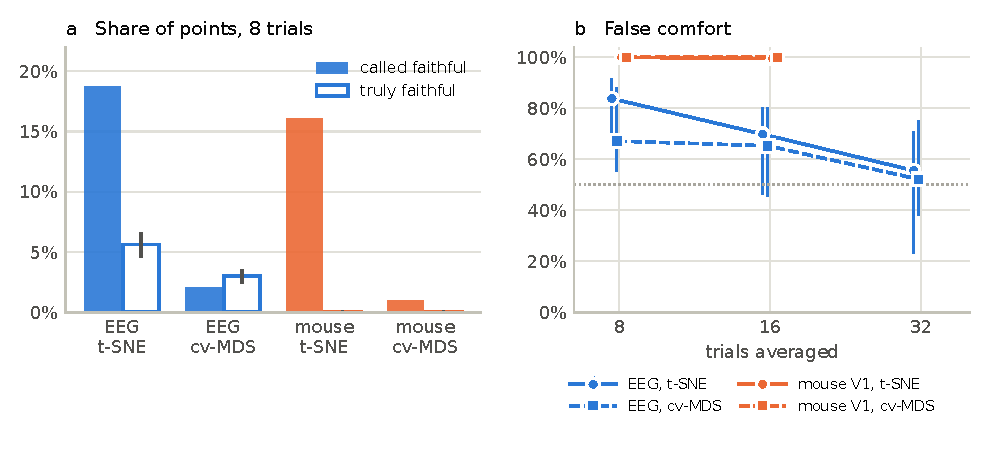
\includegraphics[width=\linewidth]{figures/fig1_false_comfort.pdf}
\caption{(a)~With 8 trials averaged, the check calls far more neighborhoods faithful than are
faithful in truth; whiskers span the two extrapolants. (b)~False comfort, the share of the
check's faithful calls that are wrong, against the number of trials averaged. Points are the
midpoint of the two extrapolants' medians over subjects; bars run from the conservative bound
$L$ to the upper end of the wider 95\% interval. The dotted line is the 50\% threshold of
claims C1 and C1-RSA.}
\label{fig:fc}
\end{figure}

In EEG with 8 trials (Table~\ref{tab:primary}, Figure~\ref{fig:fc}), the check called
\EegNFeight\% of the t-SNE neighborhoods faithful while \EegTFeight\% were faithful in truth,
so \EegFCeight\% of the passing neighborhoods were not faithful (bound \EegLeight\%) and C1 is
supported. More trials helped slowly: false comfort was \EegFCsixteen\% at 16 trials (bound
\EegLsixteen\%) and \EegFCthirtytwo\% at 32, where the bound of \EegLthirtytwo\% falls short of
C2's 25\%, so C2 is not supported. The mislabel rate stayed above 10\% at every budget, with
bounds of \EegQL, supporting C3.

In mouse V1, no displayed neighborhood was faithful in truth at 8 trials, and 0.2\% were at 16,
yet the check called \MouseNFeight\% faithful: false comfort was \MouseFCeight\% (bound
\MouseLeight\% at 8 trials, \MouseLsixteen\% at 16). C1 and C3 are supported, the latter with
bounds of \MouseQL.

Maps of cross-validated distances did not remove false comfort; they made faithful calls rare,
\EegRsaNFeight\% of points in EEG and \MouseRsaNFeight\% in mouse V1 at 8 trials, and most of
those calls were wrong: \EegRsaFCeight\% in EEG (bound \EegRsaLeight\%) and \MouseRsaFCeight\%
in mouse V1. C1-RSA is supported in both datasets.

\begin{figure}[!htb]
\centering
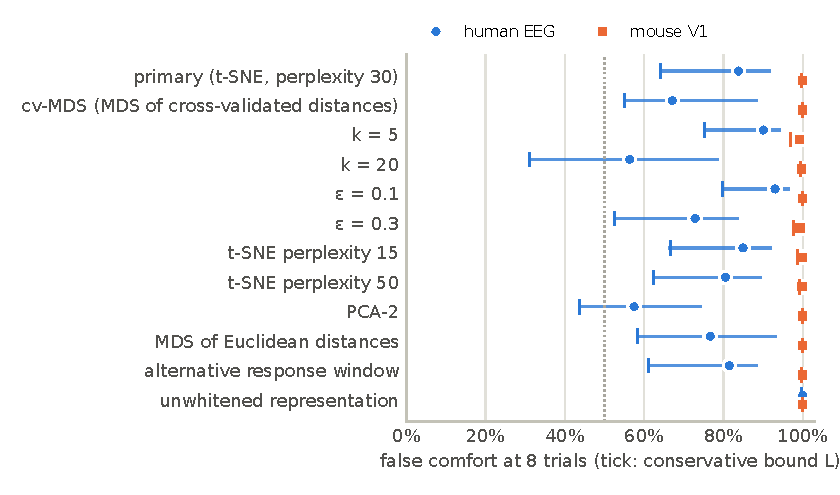
\includegraphics[width=0.8\linewidth]{figures/fig2_robustness.pdf}
\caption{False comfort at 8 trials in the 12 pre-specified variations. Markers are the midpoint
of the two extrapolants; the tick is the conservative bound $L$, which C1 requires to exceed
50\% (dotted). In EEG it does so in \EegCells{} of 12 variations, in mouse V1 in all 12.}
\label{fig:rob}
\end{figure}

Across variations (Figure~\ref{fig:rob}), C1 held in \EegCells{} of 12 in EEG and so counts as
general; it failed only on its bound for $k=20$ (estimate \EegKtwentyFC\%, bound
\EegKtwentyL\%) and for PCA-2 maps (\EegPcaFC\%, bound \EegPcaL\%). In mouse V1 it held in all
12, and the true faithful share never exceeded \MouseTFmax\%; without whitening, the check
called \MouseUnwhitenedNF\% of the mouse neighborhoods faithful and none were.

\section{Why the check fails here (exploratory)}\label{sec:why}

\begin{table}[!htb]
\centering\small
\begin{tabular}{lrr}
\toprule
 & Human EEG & Mouse V1 \\
\midrule
Image pairs with a positive cross-validated distance & 1.000 & 0.937 \\
Split-half reliability of the distance matrix & 0.879 & 0.726 \\
Distance to the 8th true neighbor, $d_{(8)}$ & 1.54 & 0.40 \\
Noise between two 16-trial means, $\sigma_{16}$ & 1.68 & 1.65 \\
Ratio $d_{(8)}/\sigma_{16}$ & 0.92 & 0.24 \\
\bottomrule
\end{tabular}

\caption{Exploratory, not pre-specified. One split per subject; medians over subjects. Blocks
$U$ and $H$ of the 20-dimensional representation: 72 repetitions in EEG, 40 in mouse V1, with
distances cross-validated between two halves. $\sigma_{16}$ is the expected noise in the
distance between two 16-trial means.}
\label{tab:snr}
\end{table}

The mouse result is not vacuous (Table~\ref{tab:snr}). Its data contain reliable image-specific
structure: \PosMouse\% of image pairs have a positive cross-validated distance, and the distance
matrix has a split-half reliability of \RelMouse. The trouble is local: the distance from an
image to its 8th nearest neighbor is only \RatioMouse{} times the noise between two 16-trial
means. The same ratio is \RatioEeg{} in EEG, where a minority of neighborhoods is faithful. In
both datasets the averaged data reproduce the global geometry while the local ordering that
neighborhood labels depend on stays inside the noise. The map, fitted to the same averages,
follows that noise, and the check, computed from the same averages, confirms it. We offer the
ratio as an account of the difference between the datasets, not as a tested claim.

\section{Discussion}\label{sec:disc}

A 2-D map of trial-averaged responses can be consistent with the averaged data, neighborhood by
neighborhood, and still say little about the responses the averaging estimates. Checking the map
against the averaged data does not guard against this: at typical budgets most neighborhoods that
pass are not faithful, and cross-validated distances make the check stricter but not accurate.
Local neighborhoods in such maps should be read only against a reference built from held-out
repetitions; the false-comfort estimate of Section~\ref{sec:est} is one, and its code is
available. Reading only neighborhoods that recur in maps of independent halves of the trials
would be cheaper, but we have not tested it, and recurrence is not the same as faithfulness to
the noise-free responses.

Lin and Fukuyama \citep{lin2024} also judge maps against a denoised signal, obtained by PCA
truncation of the same data; here the reference comes from held-out repetitions, at the level
of individual neighborhoods and as a function of the number of trials. Noise ceilings in
representational analyses \citep{nili2014,schutt2023} bound how well a model can match a whole
dissimilarity matrix, not whether neighborhoods are faithful. Downsampling studies compare
noisy neighbor graphs with a deeper reference \citep{ahlmann2023} but treat that reference as
the truth. Per-point confidence statements about neighborhoods are possible in principle through
simultaneous rank inference \citep{mogstad2024}; in a pilot on THINGS-EEG2, however, such
certificates resolved no neighborhood either way even at 72 trials, consistent with
Table~\ref{tab:snr}.

Several limitations apply. Both datasets are visual responses to images, and one neighborhood
definition ($k=10$, $\varepsilon=0.2$, $k'=2k$) was varied one factor at a time; the effect may
be weaker where neighbor distances are large relative to trial noise. The extrapolation assumes
a functional form; we report two and judge claims on the more conservative, and the plasmode
check found negligible bias, though its truth is itself a finite average. Noise shared by the
analyst's and the reference repetitions, such as slow drift, counts as signal; blocks were
balanced over sessions or halves of a session to limit it. The EEG confirmation reused the
pilot's data with new splits, and pre-specification was by commits to a version-controlled
repository rather than an external registry. Finally, the representation was noise-normalized;
without that, false comfort in EEG rose to \EegUnwhitenedFC\% at 8 trials, and in mouse V1 it
was total either way.

\section*{Data and code availability}
THINGS-EEG2 preprocessed data are available from the Open Science Framework (node
\texttt{anp5v}) \citep{gifford2022}. The Allen Brain Observatory Visual Coding data are
available from the Allen Institute's public data store under its terms of use
\citep{devries2020}. The code, the pre-specified protocols with their commit history, and all
results will be released with the paper. \todo{repository URL}

\section*{Use of AI assistance}
This work was carried out with Claude (Anthropic; model Claude Opus 5.5) as an AI research
assistant. Under the author's direction, Claude:
\begin{itemize}
  \item designed and implemented the analyses and ran them;
  \item searched and summarized the literature;
  \item drafted the text, figures and tables.
\end{itemize}
The author set the research direction, made the decisions reported here (including the choice
of datasets and every decision to run a pre-specified analysis), reviewed the analyses and the
text, and takes full responsibility for the content.

\bibliographystyle{unsrtnat}
\bibliography{refs}

\end{document}
